%pmr2350
\section{Estampagem}

\begin{itemize}
\item ferramentaas de corte
\item ferramentas de dobra
\item ferramentas de lubutimento profundo
\item ferramentas progressivas
\end{itemize}

% \begin{figure}[h]
% \begin{center}
% 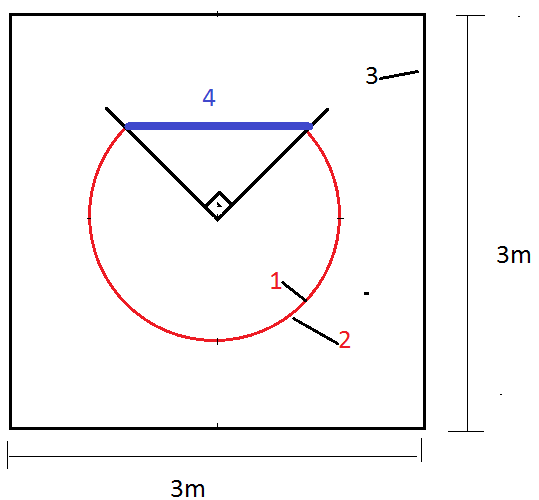
\includegraphics[scale=0.48]{./fig/1.png}
% \caption{\label{fig:1}1} 
% \end{center}
% \end{figure}

\myfig[scale=.48]{figPMR2350-20111019-01}{}

% \begin{figure}[h]
% \begin{center}
% 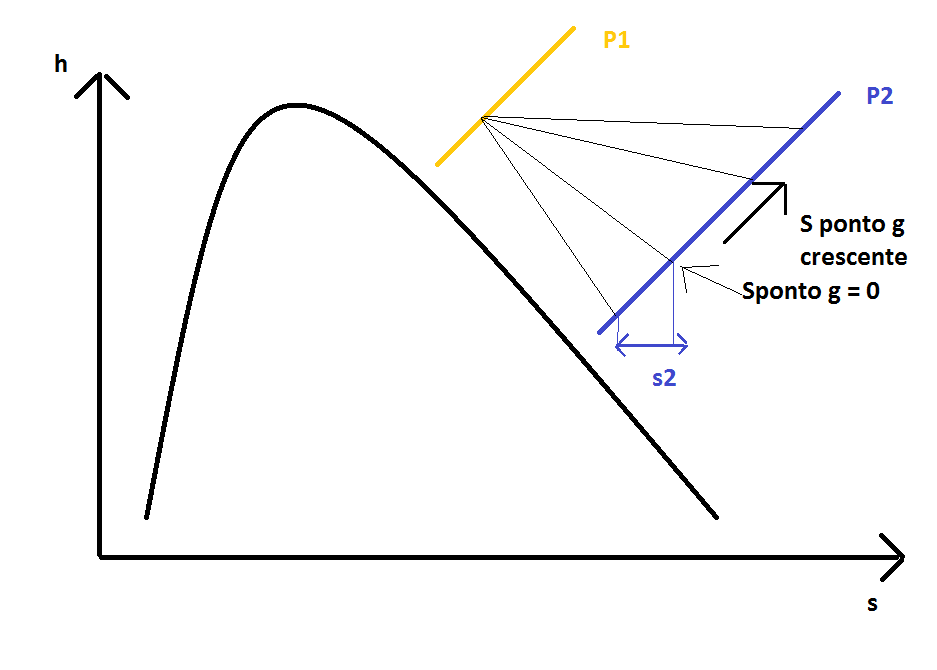
\includegraphics[scale=0.58]{./fig/2.png}
% \caption{\label{fig:1}2} 
% \end{center}
% \end{figure}

\myfig[scale=.48]{figPMR2350-20111019-02}{}

% \begin{figure}[h]
% \begin{center}
% 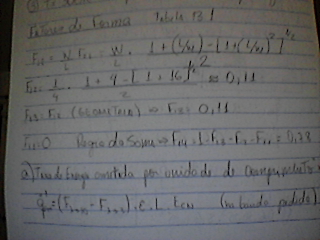
\includegraphics[scale=0.48]{./fig/3.png}
% \caption{\label{fig:1}3} 
% \end{center}
% \end{figure}

\myfig[scale=.48]{figPMR2350-20111019-03}{}

Determinação do esforço de corte ($P_{c}$)
Analogia a ResMat
\[P_{c}=K_{c}S_{c}=K_{c}*p*e\]
$K_{c}=$Resistencia ao corte(N/$m^{2}$)f(Mat, ºC)
$S_{c}$=seção do corte (mm$^{2}$)=perímetro de corte($\rho$)x espessura da chapa (e)


% \begin{figure}[h]
% \begin{center}
% 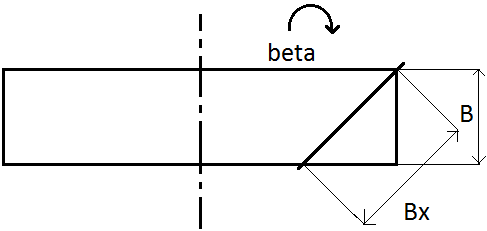
\includegraphics[scale=0.78]{./fig/4.png}
% \caption{\label{fig:1}4} 
% \end{center}
% \end{figure}

\myfig[scale=.48]{figPMR2350-20111019-04}{}

% Table generated by Excel2LaTeX from sheet 'Plan1'
\begin{table}[htbp]
  \centering
  \caption{Tolerâncias}
    \begin{tabular}{rrrrrrrrr}
    \toprule
    operação & descrição & medida nominal (mm) &       & mm    & Tolerancia Máx () &       &       & Folga (mm) \\
    \midrule
    furaçao & poncao & 10    &       &       & -0,2  &       &       & 10,2 \\
          & matriz & 10    &       &       & -0,2  &       &       & 10,3 \\
    recorte & punção & 30    &       &       & -0,2  &       &       & 29,7 \\
          & matriz & 30    &       &       & -0,2  &       &       & 29,8 \\
    \bottomrule
    \end{tabular}%
  \label{tab:addlabel}%
\end{table}